% =====================================================================
% PE-U4 — Procesamiento Distribuido con Apache Spark
% Comprobación experimental de la Ley de Amdahl
% Asignatura: Aplicaciones Distribuidas (ISR-701) — UTEQ
% Formato: IEEE doble columna (IEEEtran) + biblatex estilo IEEE (biber)
% Compilación: pdflatex -> biber -> pdflatex -> pdflatex
% Archivo principal: PE_U4_Informe.tex | Bibliografía: references_U4.bib
% =====================================================================
\documentclass[10pt,journal]{IEEEtran}

\usepackage[utf8]{inputenc}
\usepackage[T1]{fontenc}
\usepackage[spanish,es-tabla,es-noquoting]{babel}
\usepackage{amsmath}
\usepackage{graphicx}
\usepackage{booktabs}
\usepackage{siunitx}
\usepackage{listings}
\usepackage{array}
\usepackage{csquotes} % requerido por biblatex cuando se usa babel
\usepackage[backend=biber,style=ieee,sorting=none]{biblatex}



\addbibresource{references_U4.bib}

% Rutas de figuras: el documento compila desde docs/ (estructura del repositorio)
% y también desde la raíz del repositorio.
\graphicspath{{../resultados/figuras/}{../evidencia/}{resultados/figuras/}{evidencia/}{./}}

% Texto íntegramente en negro, sin bordes, sin encabezados ni pies de página,
% pero con páginas enumeradas (estilo plain: solo número de página).
\pagestyle{plain}

% Control de espacios en blanco: permite que los flotantes ocupen más
% proporción de la página y evita que LaTeX estire el texto verticalmente
% dejando huecos entre párrafos.
\renewcommand{\topfraction}{0.92}
\renewcommand{\bottomfraction}{0.85}
\renewcommand{\textfraction}{0.07}
\renewcommand{\floatpagefraction}{0.80}
\setcounter{topnumber}{3}
\setcounter{bottomnumber}{2}
\setcounter{totalnumber}{5}
\raggedbottom

% siunitx: separador decimal con coma (convención en español)
\sisetup{output-decimal-marker={,},group-separator={\,},group-minimum-digits=4}

% Reducción de overfull hbox (penalizados por la rúbrica)
\emergencystretch=1.5em
\hbadness=10000

% Configuración de listings: sin marcos ni colores (todo en negro)
\lstset{
  language=Python,
  basicstyle=\ttfamily\scriptsize,
  keywordstyle=\bfseries,
  commentstyle=\itshape,
  stringstyle=\ttfamily,
  showstringspaces=false,
  breaklines=true,
  breakatwhitespace=true,
  frame=none,
  numbers=none,
  columns=flexible,
  keepspaces=true,
  captionpos=b,
  tabsize=4
}
\renewcommand{\lstlistingname}{Listado}

\begin{document}

% =====================================================================
% PORTADA INSTITUCIONAL (una columna; no cuenta como contenido)
% =====================================================================
\onecolumn
\thispagestyle{plain}
\begin{center}
{\Large \textbf{UNIVERSIDAD T\'ECNICA ESTATAL DE QUEVEDO}}\\[0.4em]
{\large Facultad de Ciencias de la Computaci\'on}\\[0.2em]
{\large Carrera de Ingenier\'ia de Software}\\[2.0em]

{\large \textbf{Pr\'actica Experimental Unidad 4 --- GA-SUM-05 / PE-U4}}\\[0.6em]
{\LARGE \textbf{Procesamiento Distribuido con Apache Spark:\\[0.2em]
comprobaci\'on experimental de la Ley de Amdahl\\[0.2em]
aplicada al Proyecto Fin de Curso}}\\[2.0em]

\begin{tabular}{ll}
\textbf{Asignatura:} & Aplicaciones Distribuidas (ISR-701) [20701]\\[0.2em]
\textbf{Unidad:} & Unidad 4 -- C\'omputo Paralelo y Distribuido\\[0.2em]
\textbf{C\'odigo de actividad:} & GA-SUM-05 / PE-U4\\[0.2em]
\textbf{Nivel / Paralelo:} & S\'eptimo nivel -- Paralelo A\\[0.2em]
\textbf{Docente responsable:} & Gleiston C. Guerrero-Ulloa, M.Sc.\\[0.2em]
\textbf{Per\'iodo acad\'emico:} & 2026--2027 PPA\\[0.2em]
\textbf{Semana de entrega:} & Semana 14\\[0.2em]
\textbf{C\'odigo del equipo:} & Equipo C\\
\end{tabular}\\[2.0em]

{\large \textbf{PFC de referencia elegido}}\\[0.4em]
\begin{tabular}{ll}
\textbf{C\'odigo del PFC:} & FUVV\\[0.2em]
\textbf{T\'itulo del sistema:} & Sistema de Control de Laboratorios Inform\'aticos (SCLI)\\
\end{tabular}\\[2.0em]

{\large \textbf{Integrantes del equipo}}\\[0.4em]
\begin{tabular}{@{}llp{0.52\textwidth}@{}}
\toprule
\textbf{Integrante} & \textbf{PFC de origen} & \textbf{Rol asumido}\\
\midrule
Freddy Farinango & FUVV & Coordinaci\'on del equipo, despliegue del cl\'uster Spark
Standalone, protocolo experimental y redacci\'on \LaTeX\\[0.3em]
Jeremy Gaibor & FUVV & Implementaci\'on de las transformaciones T1--T5 en pandas y
PySpark, medici\'on de tiempos y redacci\'on \LaTeX\\[0.3em]
Iv\'an Villamar\'in & FUVV & An\'alisis cuantitativo, generaci\'on de figuras,
verificaci\'on de equivalencia y redacci\'on \LaTeX\\
\bottomrule
\end{tabular}\\[0.6em]
{\footnotesize La redacci\'on, estructuraci\'on y compilaci\'on del documento \LaTeX{}
fue una labor colaborativa de los tres integrantes.}
\end{center}

\vspace{1.5em}
\noindent\textbf{Justificaci\'on t\'ecnica de la elecci\'on del PFC (dominio FUVV).}
El dominio FUVV, correspondiente al Sistema de Control de Laboratorios
Inform\'aticos (SCLI), se eligi\'o porque es el dominio que con mayor naturalidad
genera vol\'umenes de datos que justifican un motor distribuido. Cada laboratorio de la
facultad produce, de manera continua, solicitudes de reserva con su ciclo de estados
(pendiente, aprobada, rechazada, cancelada, finalizada), registros de asistencia y de uso
de equipos, y eventos de monitoreo por estaci\'on de trabajo. Acumulados a lo largo de
varios per\'iodos acad\'emicos y proyectados a decenas de laboratorios con cientos de
equipos, estos flujos superan con facilidad el mill\'on de registros anuales, un volumen
para el cual el procesamiento en un solo proceso deja de ser la \'unica alternativa
razonable y en el que resulta pertinente evaluar emp\'iricamente cu\'ando un motor
distribuido como Apache Spark aporta valor y cu\'ando su sobrecarga lo penaliza. La
decisi\'on de negocio que se apoya en el pipeline implementado es la \emph{planificaci\'on
de capacidad y priorizaci\'on de reservas}: a partir del filtrado de solicitudes aprobadas
de alta ocupaci\'on (T1), de los agregados de demanda por laboratorio (T2), del cruce con
la dimensi\'on de laboratorios y sus capacidades (T3), del puntaje determinista de
prioridad (T4) y del ranking de mayor demanda (T5), la administraci\'on puede decidir qu\'e
laboratorios ampliar, en qu\'e franjas concentrar mantenimiento y qu\'e solicitudes
priorizar cuando la capacidad es insuficiente.

\vspace{1.0em}
\noindent\textbf{Repositorio del proyecto:}
\texttt{https://github.com/ffarinangog2/pe-u4-spark-equipo-c}

\clearpage

% =====================================================================
% CUERPO DEL ART\'ICULO EN DOBLE COLUMNA (formato IEEE)
% =====================================================================
\twocolumn[{%
\begin{center}
{\LARGE \textbf{Procesamiento Distribuido con Apache Spark: comprobaci\'on experimental de la Ley de Amdahl aplicada al dominio FUVV de reserva de laboratorios inform\'aticos}}\\[0.9em]
{\large Freddy Farinango, Jeremy Gaibor e Iv\'an Villamar\'in}\\[0.3em]
{\normalsize Carrera de Ingenier\'ia de Software, Facultad de Ciencias de la Computaci\'on}\\
{\normalsize Universidad T\'ecnica Estatal de Quevedo, Quevedo, Ecuador}\\[0.3em]
{\normalsize Aplicaciones Distribuidas (ISR-701) --- Docente: Gleiston C. Guerrero-Ulloa, M.Sc. --- Per\'iodo 2026--2027 PPA}\\[1.4em]
\end{center}
}]

\section*{Resumen}
Esta pr\'actica comprueba experimentalmente la Ley de Amdahl mediante la
implementaci\'on y medici\'on de un pipeline de cinco transformaciones de datos
(T1--T5) ejecutado de forma secuencial con pandas y de forma distribuida con
PySpark 3.5.0 sobre un cl\'uster Spark Standalone real, utilizando un conjunto de
datos sint\'etico y reproducible de \num{500000} solicitudes de reserva de
laboratorios del dominio FUVV. Cada transformaci\'on se midi\'o con
\texttt{time.perf\_counter()} en cinco repeticiones tras una ejecuci\'on de
calentamiento descartada, reportando la mediana. Con cuatro executors, PySpark
super\'o a pandas solo en las transformaciones intensivas por fila (T4, con
speedup de \num{1.2519}, y T5, con \num{1.1244}), mientras que en T1, T2 y T3 el
speedup fue inferior a la unidad debido a la sobrecarga de planificaci\'on y
\emph{shuffle} del motor. El escalado de T3 con 1, 2 y 4 executors arroj\'o
speedups de \num{1.0000}, \num{1.9217} y \num{1.5727}; aplicando la forma inversa
de la Ley de Amdahl (m\'etrica de Karp-Flatt) se obtuvo una fracci\'on no
escalable observada de $f = \num{0.5145}$, que impone un l\'imite te\'orico
m\'aximo de $S_{\text{m\'ax}} = \num{1.9437}$ alcanzable con infinitos
procesadores. Los resultados confirman cuantitativamente que el l\'imite de la
paralelizaci\'on lo fija la fracci\'on serial y que, para el volumen evaluado, el
motor distribuido solo es rentable en transformaciones con c\'omputo por registro
suficientemente costoso.

\section*{Palabras clave}
Ley de Amdahl; Apache Spark; PySpark; pandas; speedup; fracci\'on serial;
eficiencia paralela; Gustafson-Barsis; procesamiento distribuido; benchmarking.

\section{Introducci\'on}
El c\'omputo paralelo y distribuido constituye hoy la v\'ia dominante para
procesar vol\'umenes de datos que exceden la capacidad de un solo proceso, pero
su adopci\'on no es gratuita: todo motor distribuido introduce costos de
planificaci\'on, serializaci\'on, transferencia y coordinaci\'on que compiten con
la ganancia del paralelismo. La Ley de Amdahl formaliz\'o tempranamente este
compromiso al demostrar que el speedup alcanzable por un programa est\'a acotado
por su fracci\'on estrictamente serial, independientemente del n\'umero de
procesadores disponibles \cite{amdahl1967}. D\'ecadas despu\'es, la reformulaci\'on
de Gustafson-Barsis matiz\'o esa cota para escenarios en los que la carga de
trabajo crece con los recursos \cite{gustafson1988}, y la m\'etrica de Karp-Flatt
propuso estimar emp\'iricamente la fracci\'on serial a partir de mediciones
reales \cite{karp1990}.

Esta pr\'actica experimental cierra el recorrido conceptual de la Unidad 4 de la
asignatura Aplicaciones Distribuidas conectando cuatro capas: el modelo te\'orico
de l\'imites de paralelizaci\'on \cite{amdahl1967}, \cite{gustafson1988}; el
paradigma MapReduce que populariz\'o el procesamiento por lotes a gran escala
\cite{dean2008}; el motor unificado Apache Spark, que super\'o a MapReduce para
cargas iterativas mediante el modelo RDD en memoria \cite{zaharia2016}; y los modelos de computaci\'on en la nube sobre los que estos
motores se despliegan en producci\'on \cite{mell2011}.

El experimento se ancla en un dominio de aplicaci\'on concreto: el PFC de
referencia FUVV, Sistema de Control de Laboratorios Inform\'aticos (SCLI). El pipeline implementado no es un ejercicio abstracto sino la
versi\'on anal\'itica de una necesidad real del dominio: filtrar las
solicitudes aprobadas de alta ocupaci\'on, agregar la demanda por laboratorio,
cruzarla con la capacidad instalada, puntuar la prioridad de cada solicitud y
producir el ranking de mayor demanda que alimenta las decisiones de
planificaci\'on de capacidad. Medir ese pipeline en dos motores y confrontar
las mediciones con el modelo formal permite responder una pregunta de
ingenier\'ia que el PFC deber\'a enfrentar: a partir de qu\'e volumen, y con
cu\'antos recursos, conviene distribuir el procesamiento.

El objetivo general es comprobar experimentalmente la Ley de Amdahl
implementando y midiendo el rendimiento de un pipeline distribuido de datos con
Apache Spark sobre un conjunto de \num{500000} registros del dominio FUVV,
compar\'andolo con el procesamiento secuencial equivalente en pandas. Los
objetivos espec\'ificos son: (i) implementar las mismas cinco transformaciones
con pandas y con PySpark; (ii) medir los tiempos con precisi\'on de
microsegundos, con cinco repeticiones por transformaci\'on y reporte de la
mediana; (iii) calcular el speedup experimental y compararlo con el speedup
te\'orico de Amdahl; y (iv) determinar la fracci\'on serial observada y el
l\'imite pr\'actico de paralelizaci\'on.

El resto del documento se organiza as\'i: la Secci\'on~\ref{sec:fundamento}
desarrolla el fundamento te\'orico de la unidad; la
Secci\'on~\ref{sec:procedimiento} describe el procedimiento aplicado, el
entorno, el conjunto de datos y el protocolo de medici\'on; la
Secci\'on~\ref{sec:resultados} presenta los resultados experimentales con el
trabajo matem\'atico expl\'icito del an\'alisis de Amdahl; la
Secci\'on~\ref{sec:analisis} discute cr\'iticamente los hallazgos, incluida la
anomal\'ia de escalado entre dos y cuatro executors; la
Secci\'on~\ref{sec:preguntas} responde las preguntas obligatorias del Anexo A de
la gu\'ia; y la Secci\'on~\ref{sec:conclusiones} recoge las conclusiones
individuales de los integrantes.

\section{Fundamento te\'orico}
\label{sec:fundamento}

\subsection{Fundamentos de paralelismo y Ley de Amdahl}
\label{sec:amdahl}
El paralelismo busca reducir el tiempo de resoluci\'on de un problema
repartiendo trabajo entre varias unidades de procesamiento, y se manifiesta en
dos formas complementarias. El \emph{paralelismo de datos} aplica la misma
operaci\'on simult\'aneamente sobre particiones disjuntas de un conjunto de
datos, y es el modelo natural de los motores de procesamiento masivo como
MapReduce y Spark, en los que cada tarea procesa una partici\'on del conjunto
\cite{dean2008}, \cite{zaharia2016}. El \emph{paralelismo de tareas}, en cambio,
ejecuta simult\'aneamente operaciones distintas, posiblemente sobre los mismos
datos, y aparece en Spark en la ejecuci\'on concurrente de etapas independientes
del grafo de ejecuci\'on \cite{zaharia2016}, \cite{armbrust2015}. En ambos casos
la ganancia est\'a limitada por la porci\'on del trabajo que no puede repartirse.

Amdahl formul\'o en 1967 el argumento cuantitativo cl\'asico sobre ese
l\'imite \cite{amdahl1967}. Sea $T_1$ el tiempo de ejecuci\'on con una unidad de
procesamiento, $p$ la fracci\'on del tiempo que corresponde a trabajo
paralelizable y $(1-p)$ la fracci\'on estrictamente serial. Con $N$ unidades, la
parte paralelizable idealmente se reduce a $p\,T_1/N$, mientras que la serial
permanece invariante, de modo que
$T_N = (1-p)\,T_1 + \frac{p}{N}\,T_1$. El speedup, definido como
$S(N) = T_1 / T_N$, resulta
\begin{equation}
S(N) \;=\; \frac{1}{(1-p) + \dfrac{p}{N}},
\label{eq:amdahl}
\end{equation}
que es la Ley de Amdahl \cite{amdahl1967}, \cite{karp1990}. Tomando el l\'imite
cuando $N \to \infty$, el t\'ermino $p/N$ se anula y el speedup m\'aximo queda
fijado exclusivamente por la fracci\'on serial:
\begin{equation}
S_{\text{m\'ax}} \;=\; \lim_{N \to \infty} S(N) \;=\; \frac{1}{1-p}.
\label{eq:smax}
\end{equation}
La consecuencia pr\'actica de \eqref{eq:smax} es severa: con apenas un
\SI{10}{\percent} de c\'odigo serial ($p=0{,}9$), ning\'un n\'umero de
procesadores puede superar un speedup de 10.

Gustafson observ\'o que en la pr\'actica cient\'ifica el tama\~no del problema
crece con los recursos disponibles: no se resuelve el mismo problema m\'as
r\'apido, sino un problema mayor en el mismo tiempo \cite{gustafson1988}.
Manteniendo fija la fracci\'on serial del tiempo de ejecuci\'on paralelo, el
speedup escalado de Gustafson-Barsis es
\begin{equation}
S_G(N) \;=\; N - (1-p)\,(N-1),
\label{eq:gustafson}
\end{equation}
una recta creciente en $N$ que no presenta la saturaci\'on de
\eqref{eq:amdahl} y que resulta el modelo adecuado cuando la carga escala con el
cl\'uster \cite{gustafson1988}, \cite{karp1990}.

Despejando $p$ de \eqref{eq:amdahl} para una medici\'on experimental con $N$
unidades y speedup observado $S$, se obtiene la fracci\'on serial impl\'icita,
que es la m\'etrica de Karp-Flatt en su forma equivalente \cite{karp1990}:
\begin{equation}
f \;=\; 1-p \;=\; \frac{\dfrac{1}{S} - \dfrac{1}{N}}{1 - \dfrac{1}{N}},
\qquad N > 1.
\label{eq:karpflatt}
\end{equation}
Finalmente, la eficiencia del paralelismo mide qu\'e proporci\'on de la
capacidad agregada se aprovecha realmente:
\begin{equation}
E(N) \;=\; \frac{S(N)}{N}.
\label{eq:eficiencia}
\end{equation}

La eficiencia \eqref{eq:eficiencia} tiene su propia lectura asint\'otica: como
$S(N)$ satura en $1/(1-p)$, la eficiencia $E(N) = S(N)/N$ tiende a cero cuando
$N$ crece, de modo que todo sistema de talla fija termina desperdiciando la
mayor parte de su capacidad agregada si se sobredimensiona \cite{amdahl1967},
\cite{karp1990}. De ah\'i se deriva una regla de dise\~no que esta pr\'actica
comprueba emp\'iricamente: el n\'umero \'optimo de unidades de procesamiento no
es el m\'aximo disponible, sino el mayor $N$ para el cual la eficiencia se
mantiene por encima de un umbral aceptable, t\'ipicamente entre el
\SI{70}{\percent} y el \SI{90}{\percent}. Karp y Flatt a\~naden el uso
diagn\'ostico de \eqref{eq:karpflatt}: si al medir con valores crecientes de
$N$ la fracci\'on serial experimental permanece constante, la p\'erdida de
eficiencia se debe al paralelismo limitado del algoritmo; si $f$ crece con $N$,
la causa es la sobrecarga creciente del sistema (planificaci\'on,
comunicaci\'on, contenci\'on), un s\'intoma que exige optimizar la plataforma y
no reescribir el algoritmo \cite{karp1990}.

Es indispensable una advertencia metodol\'ogica sobre \eqref{eq:karpflatt}: la
magnitud despejada a partir de mediciones no es la fracci\'on serial
\emph{algor\'itmica}, sino la fracci\'on \emph{no escalable observada}, que
agrega a la porci\'on serial del algoritmo toda la sobrecarga de
planificaci\'on, serializaci\'on, comunicaci\'on y \emph{shuffle} del motor de
ejecuci\'on \cite{karp1990}, \cite{ahmed2020}. Confundir ambas conduce a
subestimar sistem\'aticamente el potencial de paralelizaci\'on del algoritmo
puro. La Fig.~\ref{fig:curvas} representa \eqref{eq:amdahl} para fracciones
paralelizables $p = 0{,}5$; $0{,}75$; $0{,}9$ y $0{,}95$, y evidencia
gr\'aficamente la saturaci\'on que impone \eqref{eq:smax}: las cuatro curvas se
aplanan hacia as\'intotas de valor $2$, $4$, $10$ y $20$ respectivamente, de
modo que a\~nadir procesadores m\'as all\'a de cierto punto produce ganancias
marginales despreciables.

\begin{figure}[!t]
\centering
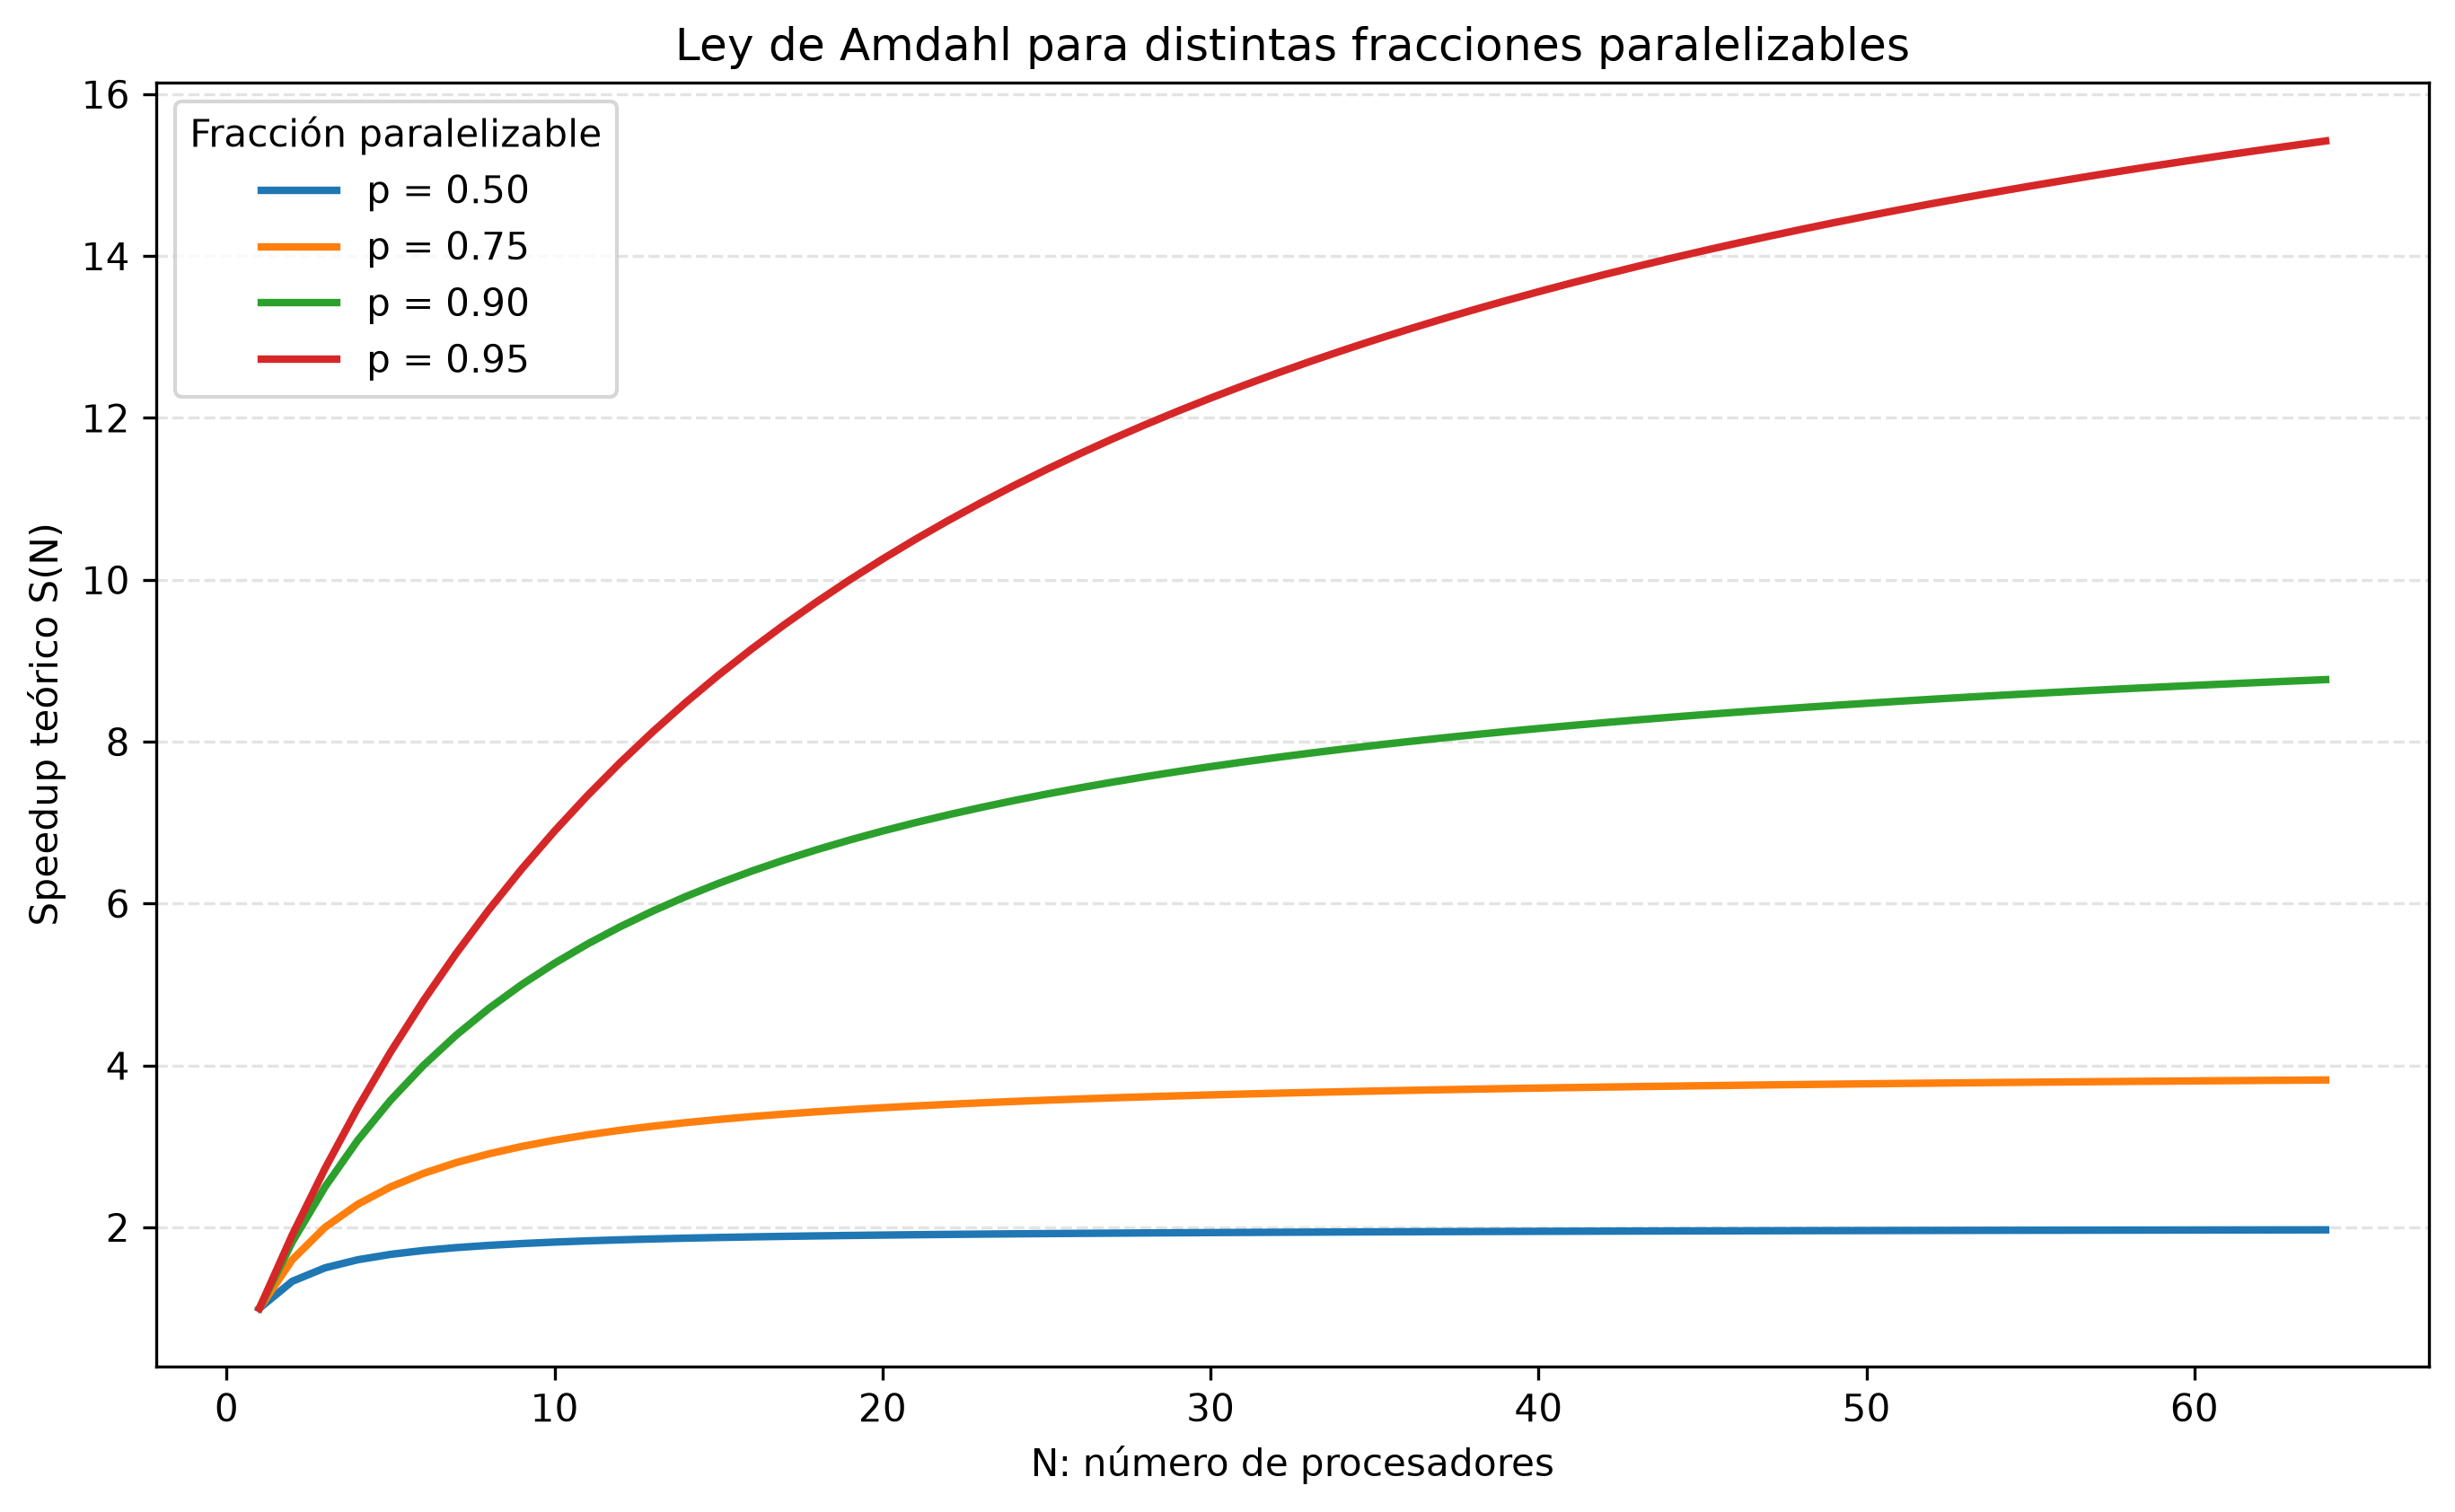
\includegraphics[width=\columnwidth]{07_curvas_amdahl_fracciones.png}
\caption{Speedup te\'orico de Amdahl seg\'un \eqref{eq:amdahl} frente al
n\'umero de procesadores $N$ para fracciones paralelizables
$p = 0{,}5$; $0{,}75$; $0{,}9$ y $0{,}95$. Cada curva satura en la as\'intota
$1/(1-p)$ dada por \eqref{eq:smax}. Figura generada con matplotlib por el
script \texttt{src/graficas.py} del repositorio.}
\label{fig:curvas}
\end{figure}

\subsection{Paradigma MapReduce y Apache Hadoop}
\label{sec:mapreduce}
MapReduce es el modelo de programaci\'on propuesto por Dean y Ghemawat en Google
para procesar grandes conjuntos de datos sobre cl\'usteres de m\'aquinas
convencionales, ocultando al programador los detalles de particionamiento,
planificaci\'on, tolerancia a fallos y comunicaci\'on \cite{dean2008}.
Formalmente, el usuario define dos funciones. La funci\'on
$\mathit{map}: (k_1, v_1) \rightarrow \mathit{list}(k_2, v_2)$ procesa cada par
clave--valor de entrada y emite pares intermedios; la funci\'on
$\mathit{reduce}: (k_2, \mathit{list}(v_2)) \rightarrow \mathit{list}(v_3)$
recibe todos los valores intermedios asociados a una misma clave y los combina
en el resultado final \cite{dean2008}, \cite{shvachko2010}. El flujo completo de
ejecuci\'on consta de cinco fases: \emph{split}, en la que la entrada se divide
en fragmentos; \emph{map}, en la que cada fragmento se procesa en paralelo;
\emph{shuffle}, en la que los pares intermedios se redistribuyen por clave entre
los nodos; \emph{sort}, en la que cada nodo ordena las claves recibidas; y
\emph{reduce}, en la que se agregan los valores por clave \cite{dean2008}.

Apache Hadoop es la implementaci\'on de c\'odigo abierto de este modelo y se
apoya en dos subsistemas. HDFS es un sistema de archivos distribuido que divide
cada archivo en bloques de gran tama\~no y los replica, por defecto tres veces,
entre nodos de datos coordinados por un nodo de nombres que mantiene los
metadatos; la replicaci\'on proporciona a la vez tolerancia a fallos de disco y
de nodo y oportunidades de \emph{localidad de datos}, es decir, de planificar
cada tarea map en un nodo que ya alberga una r\'eplica de su bloque, evitando
transferirlo por la red \cite{shvachko2010}, \cite{white2015}. YARN, por su parte, separa la
gesti\'on de recursos de la l\'ogica de las aplicaciones: un gestor de recursos
global negocia contenedores de CPU y memoria con los gestores de nodo, y cada
aplicaci\'on ejecuta su propio maestro que solicita contenedores y supervisa
sus tareas, lo que permite que MapReduce, Spark y otros motores convivan en el
mismo cl\'uster \cite{vavilapalli2013}. Frente al procesamiento tradicional en un
solo servidor, el modelo ofrece escalabilidad horizontal casi lineal para
cargas por lotes, tolerancia a fallos mediante reejecuci\'on determinista de
tareas fallidas y ocultamiento completo de la distribuci\'on al programador
\cite{dean2008}, \cite{white2015}, \cite{shvachko2010}.

Su limitaci\'on central aparece en el procesamiento \emph{iterativo}: cada
iteraci\'on es un trabajo MapReduce independiente que materializa sus resultados
en disco, de modo que algoritmos que reutilizan datos entre iteraciones pagan en
cada ciclo el costo completo de lectura y escritura en HDFS \cite{zaharia2016},
\cite{shvachko2010}. La evidencia emp\'irica publicada confirma esta brecha: en el
estudio sistem\'atico de Ahmed \emph{et al.} con la suite HiBench, Spark
super\'o a Hadoop en la mayor\'ia de las cargas evaluadas, con ventajas
especialmente amplias en cargas iterativas de aprendizaje autom\'atico, aunque
la magnitud de la ventaja depende de la carga y de la configuraci\'on del
cl\'uster \cite{ahmed2020}. Este resultado arbitrado, y no material
promocional, es el que sustenta en este informe toda comparaci\'on de
rendimiento entre ambos motores \cite{ahmed2020}, \cite{zaharia2016}.

\subsection{Apache Spark: arquitectura y modelo de programaci\'on}
\label{sec:spark}
Apache Spark es un motor unificado de procesamiento de datos a gran escala cuya
arquitectura distingue tres componentes \cite{zaharia2016}, \cite{armbrust2015}:
el \emph{driver}, proceso que ejecuta el programa del usuario, construye el plan
de ejecuci\'on y coordina el trabajo; el \emph{cluster manager} (Standalone,
YARN, Mesos o Kubernetes), que asigna recursos f\'isicos; y los
\emph{executors}, procesos JVM distribuidos que ejecutan tareas sobre
particiones de datos y cachean resultados en memoria. En esta pr\'actica se
emple\'o el gestor Standalone propio de Spark con executors expl\'icitamente
registrados, lo que permite controlar $N$ en el experimento.

La abstracci\'on fundacional del motor es el RDD (\emph{Resilient Distributed
Dataset}): una colecci\'on de solo lectura, particionada entre los nodos, que
registra el \emph{lineage} de transformaciones gruesas con que fue construida
\cite{zaharia2012}, \cite{zaharia2016}. La tolerancia a fallos no requiere replicar los datos: ante
la p\'erdida de una partici\'on, el motor la reconstruye reaplicando el lineage
sobre los datos de origen, un mecanismo m\'as barato que la replicaci\'on de
HDFS para c\'omputo en memoria \cite{zaharia2016}. Las
transformaciones se clasifican en \emph{estrechas}, en las que cada partici\'on
de salida depende de una sola partici\'on de entrada (filtros, proyecciones,
columnas derivadas), y \emph{anchas}, en las que una partici\'on de salida
depende de muchas de entrada y exige redistribuir datos por la red mediante
shuffle (agrupaciones, joins particionados, ordenamientos globales)
\cite{zaharia2012}, \cite{chambers2018}; la distinci\'on es central para este
experimento, porque T1 y T4 son estrechas mientras que T2, T3 y T5 son anchas,
y el costo del shuffle es precisamente el componente de sobrecarga que la
fracci\'on no escalable observada captura. Sobre los RDD se construyen las API
de DataFrames, colecciones con esquema relacional expl\'icito, y Datasets, su
variante con tipado est\'atico en Scala y Java; ambas delegan en el optimizador
Catalyst, que aplica reglas de reescritura al plan l\'ogico (poda de columnas,
empuje de predicados hacia la fuente, reordenaci\'on y elecci\'on de estrategia
de join) antes de generar el plan f\'isico \cite{armbrust2015}. Precisamente por la acci\'on de Catalyst, las
transformaciones sobre DataFrames no se ejecutan en el orden en que se
escriben: el plan l\'ogico declarado se reescribe antes de ejecutarse, y por
ello la Spark UI muestra un DAG que no coincide literalmente con el texto del
programa \cite{armbrust2015}.

El modelo de ejecuci\'on es perezoso: las \emph{transformaciones} (filter,
select, groupBy, join) solo declaran el plan, y \'unicamente las
\emph{acciones} (count, collect, write) disparan la ejecuci\'on
\cite{zaharia2016}, \cite{armbrust2015}. Al invocarse una acci\'on, el driver
compila el lineage en un DAG de \emph{stages} delimitados por las fronteras de
shuffle; cada stage se descompone en \emph{tasks}, una por partici\'on, que el
planificador distribuye entre los executors \cite{zaharia2016},
\cite{armbrust2015}. Esta materializaci\'on expl\'icita es la raz\'on
metodol\'ogica por la que en este experimento cada medici\'on de PySpark fuerza
una acci\'on: sin ella se medir\'ia solo la construcci\'on del plan. En cuanto a
rendimiento comparado, Spark evita la materializaci\'on a disco entre etapas
que impone MapReduce, y la evidencia emp\'irica de benchmarking le atribuye
ventajas consistentes, especialmente en cargas iterativas \cite{ahmed2020},
\cite{zaharia2016}.

\subsection{Computaci\'on en la nube: modelos y proveedores}
\label{sec:nube}
El NIST define la computaci\'on en la nube como un modelo que habilita acceso
ubicuo, conveniente y bajo demanda a un conjunto compartido de recursos de
c\'omputo configurables, aprovisionables con m\'inimo esfuerzo de gesti\'on, y
enumera cinco caracter\'isticas esenciales: autoservicio bajo demanda, amplio
acceso por red, agrupaci\'on de recursos, elasticidad r\'apida y servicio medido
\cite{mell2011}. Sobre esa base distingue los modelos de servicio IaaS, PaaS y
SaaS, seg\'un el nivel de la pila que gestiona el proveedor \cite{mell2011}; la
industria a\~nadi\'o posteriormente FaaS, en el que la unidad de despliegue es
la funci\'on y el proveedor gestiona todo el ciclo de ejecuci\'on, extensi\'on
natural de la elasticidad y del pago por uso que la literatura fundacional de
la nube identific\'o como sus rasgos econ\'omicos distintivos
\cite{armbrust2010}.

Las cinco caracter\'isticas esenciales merecen glosa porque explican por qu\'e
los motores distribuidos migraron a la nube. El \emph{autoservicio bajo
demanda} elimina la negociaci\'on humana del aprovisionamiento; el \emph{amplio
acceso por red} desacopla el consumo del lugar; la \emph{agrupaci\'on de
recursos} permite al proveedor multiplexar clientes sobre el mismo hardware con
econom\'ias de escala; la \emph{elasticidad r\'apida} habilita crecer y
decrecer el cl\'uster al ritmo de la carga, condici\'on necesaria para que el
r\'egimen de Gustafson sea alcanzable en la pr\'actica; y el \emph{servicio
medido} convierte el c\'omputo en costo variable, lo que hace del
sobredimensionamiento un despilfarro contable inmediato \cite{mell2011}. En los
modelos de servicio, IaaS entrega m\'aquinas virtuales y redes sobre las que el
usuario instala el motor; PaaS entrega el motor gestionado; SaaS entrega la
aplicaci\'on final; y FaaS entrega ejecuci\'on de funciones dirigida por
eventos sin gesti\'on de servidores \cite{mell2011}, \cite{burns2024},
\cite{armbrust2010}.

Para el procesamiento distribuido, los tres grandes proveedores ofrecen
servicios gestionados equivalentes que despliegan cl\'usteres Spark/Hadoop sin
administraci\'on manual: EMR en AWS, HDInsight en Azure y Dataproc en GCP. Los
tres siguen el patr\'on PaaS sobre infraestructura el\'astica: el usuario
declara tama\~no y tipo de nodos y el proveedor gestiona aprovisionamiento,
parcheo y escalado, diferenci\'andose principalmente en el ecosistema que los
rodea (almacenamiento de objetos, cat\'alogos de datos y servicios de an\'alisis
integrados de cada nube) y en la granularidad de la facturaci\'on
\cite{mell2011}, \cite{burns2024}. El dimensionamiento de
recursos para flujos de trabajo basados en DAG, como los de Spark, es en s\'i
mismo un problema de optimizaci\'on costo--rendimiento: la literatura arbitrada
propone recomendadores que, dado un flujo y un objetivo de plazo, seleccionan
tipo y n\'umero de instancias minimizando el costo monetario, precisamente
